\documentclass{../common/SCNU_Experimental_Report}

% 填写报告头信息
\studentname{Tommy}
\studentid{20240110}
\major{Github}
\class{24级01班}
\coursename{模式识别与机器学习}
\projectname{k 近邻算法和决策树}
\verify
\experimentdate{2024年1月10日}
\teacher{Tommy}

\begin{document}
\maketitle

\section{实验原理}
\subsection{k 近邻算法}
k 近邻（k-Nearest Neighbors, kNN）是一种基本的分类与回归方法。本实验采用 kNN 进行分类，其基本思想是：对于一个新的输入实例，在训练数据集中找到与该实例最邻近的 \(k\) 个实例，这 \(k\) 个实例的多数所属的类别即为该输入实例的类别。

距离度量采用欧氏距离（\(L_2\) 距离），对于两个 \(n\) 维样本 \(x_i = (x_i^{(1)}, x_i^{(2)}, ..., x_i^{(n)})^T\) 和 \(x_j = (x_j^{(1)}, x_j^{(2)}, ..., x_j^{(n)})^T\)，其欧氏距离定义为：
\[
    L_2(x_i, x_j) = \left( \sum_{l=1}^n |x_i^{(l)} - x_j^{(l)}|^2 \right)^{\frac{1}{2}}
\]

为了提高泛化能力，本实验采用 5 折交叉验证选择最优的 \(k\) 值，并扩展实现了曼哈顿距离（\(L_1\) 距离）作为对比。

\subsection{决策树}
决策树是一种基于树结构的分类模型，每个内部节点表示一个特征上的测试，每个分支代表一个测试输出，每个叶节点代表一个类别。本实验实现 ID3 算法和 C4.5 算法。

核心概念包括：
\begin{itemize}
    \item \textbf{信息熵}：度量数据集的不确定性。对于数据集 \(D\)，其熵为：
          \[
              H(D) = -\sum_{k=1}^{K} \frac{|C_k|}{|D|} \log_2 \frac{|C_k|}{|D|}
          \]
          其中 \(K\) 为类别数，\(|C_k|\) 为第 \(k\) 类样本数。
    \item \textbf{条件熵}：在已知特征 \(A\) 的条件下，数据集 \(D\) 的不确定性：
          \[
              H(D|A) = \sum_{i=1}^{n} \frac{|D_i|}{|D|} H(D_i)
          \]
    \item \textbf{信息增益}：特征 \(A\) 带来的不确定性减少量：
          \[
              g(D, A) = H(D) - H(D|A)
          \]
          ID3 算法选择信息增益最大的特征进行划分。
    \item \textbf{信息增益比}：为解决 ID3 偏向取值较多特征的问题，C4.5 算法采用信息增益比：
          \[
              g_R(D, A) = \frac{g(D, A)}{H_A(D)}, \quad H_A(D) = -\sum_{i=1}^{n} \frac{|D_i|}{|D|} \log_2 \frac{|D_i|}{|D|}
          \]
\end{itemize}

\section{关键代码}
\subsection{k 近邻算法}
\begin{enumerate}
    \item \textbf{实验1.1：使用 print 功能观察数据}

          \begin{lstlisting}[language=Python]
# 加载鸢尾花数据集
iris_data = load_iris() # 从 sklearn 加载鸢尾花数据集
X = iris_data.data      # 提取特征矩阵，shape: (150, 4)，4个特征分别为花萼长、花萼宽、花瓣长、花瓣宽
y = iris_data.target    # 提取标签向量，shape: (150,)，0=Setosa, 1=Versicolour, 2=Virginica

# 使用 print 观察数据结构
print(f"特征数据 X:\n{X}")  # 打印所有特征值，观察数据范围和分布
print(f"标签数据 y:\n{y}")  # 打印标签，观察三类样本的分布情况
\end{lstlisting}

    \item \textbf{实验1.2：调整画图函数的参数}

          \begin{lstlisting}[language=Python]
# 可视化特征 1（花萼长度）和特征 2（花萼宽度）
plt.figure(1, figsize=(8, 6))   # 创建画布，编号为1，设置图像大小为8×6英寸
plt.scatter(X[:, 0], X[:, 1], c=y, cmap=plt.cm.Set1, edgecolor="k")
# X[:, 0] 取所有样本的第1个特征（花萼长度）
# X[:, 1] 取所有样本的第2个特征（花萼宽度）
# c=y 根据标签值设置不同颜色，使不同类别的点颜色不同
# cmap=plt.cm.Set1 使用 Set1 颜色映射方案
# edgecolor="k" 设置散点边缘为黑色，增强对比度

plt.xlabel("Sepal length")  # 设置 x 轴标签为"花萼长度"
plt.ylabel("Sepal width")   # 设置 y 轴标签为"花萼宽度"
fig1_path = ex1_path + "\\figures\\Ex1_Fig1.jpg"    # 定义图片保存路径
plt.savefig(fig1_path)  # 将图像保存到指定路径
plt.show()              # 在屏幕上显示图像

# 实验 2: 调整画图中的参数 -- colormap, edgecolor, marker 等
plt.figure(2, figsize=(8, 6))   # 创建第二个画布，大小为8×6英寸
plt.scatter(X[:, 0], y, cmap=plt.cm.Set2, edgecolor="k")
# X[:, 0] 取花萼长度作为 x 轴
# y 取标签值作为 y 轴，可视化特征与类别的关系
# cmap=plt.cm.Set2 更换为 Set2 颜色映射
# edgecolor="k" 点边缘设为黑色

plt.xlabel("Sepal length")  # x 轴标签
plt.ylabel("class")         # y 轴标签为"类别"
fig2_path = ex1_path + "\\figures\\Ex1_Fig2.jpg"    # 定义图片保存路径
plt.savefig(fig2_path)  # 将图像保存到指定路径
plt.show()              # 在屏幕上显示图像
\end{lstlisting}

    \item \textbf{扩展实验1.3：距离更改为曼哈顿距离的代码}

          \begin{lstlisting}[language=Python]
def compute_manhattan_distance(X_test, X_train):
    """
    拓展实验 1: 计算测试集与训练集之间的曼哈顿距离
    参数:
        X_test: 测试集 (n_test_samples, n_features)
        X_train: 训练集 (n_train_samples, n_features)
    返回:
        距离矩阵 (n_test_samples, n_train_samples)
    """
    # 扩展维度以便广播计算，避免显式循环
    test_squared = X_test[:, np.newaxis, :]     # shape: (n_test, 1, n_features)，在中间插入新维度
    train_squared = X_train[np.newaxis, :, :]   # shape: (1, n_train, n_features)，在开头插入新维度
    # 计算曼哈顿距离：L1 = sum(|x_i - x_j|)
    distances = np.sum(np.abs(test_squared - train_squared), axis=2)
    # np.abs() 计算绝对差值
    # np.sum(axis=2) 沿特征维度求和，得到距离矩阵
    return distances
\end{lstlisting}
\end{enumerate}

\subsection{决策树}
\begin{enumerate}
    \item \textbf{实验2.1：ID3 算法（计算条件熵，信息增益）}

          \begin{lstlisting}[language=Python]
def id3_algo(data, label):
    """
    根据信息增益选择最佳划分特征 (ID3 算法)
    参数:
        data: 数据集 (DataFrame)
        label: 标签列名称
    返回:
        max_info_gain: 最大信息增益
        best_feature: 最佳特征名称
        best_splited: 根据最佳特征划分后的子集字典
    """
    # Step 1: 计算整个数据集的熵 H(D)
    entropy_d = compute_entropy(data[label])    # 调用熵函数，计算原始数据集的不确定性
    
    # Step 2: 获取所有特征列（排除标签列）
    features = [col for col in data.columns if col not in [label]]  # 列表推导式，提取特征名
    
    # Step 3: 初始化最优变量
    max_info_gain = -float("inf")   # 初始化为负无穷，确保任何信息增益都能更新
    best_feature = None             # 记录最佳特征名称
    best_splited = None             # 记录最佳划分结果
    
    # Step 4: 遍历每个特征，计算信息增益
    for feature in features:
        # 根据当前特征划分数据集，得到不同取值对应的子集
        splited_set = split_dataframe(data, feature)
        
        # Step 4.1: 计算条件熵 H(D|A) = Σ(|D_i|/|D| * H(D_i))
        entropy_da = 0  # 初始化条件熵为0
        for _, subset in splited_set.items():   # 遍历每个子集
            if len(subset) > 0:                 # 确保子集非空
                # 计算子集的熵 H(D_i)
                entropy_di = compute_entropy(subset[label])
                # 加权求和：子集大小占比 × 子集熵
                entropy_da += len(subset) / len(data) * entropy_di
        
        # Step 4.2: 计算信息增益 g(D,A) = H(D) - H(D|A)
        info_gain = entropy_d - entropy_da
        
        # Step 5: 更新最佳特征（选择信息增益最大的）
        if info_gain > max_info_gain:
            max_info_gain = info_gain
            best_feature = feature
            best_splited = splited_set
    
    return max_info_gain, best_feature, best_splited
\end{lstlisting}

    \item \textbf{扩展实验2.2：C4.5 算法}

          \begin{lstlisting}[language=Python]
def c4_5_algo(data, label):
    """
    根据信息增益比选择最佳划分特征 (C4.5算法)
    参数:
        data: 数据集 (DataFrame)
        label: 标签列名称
    返回:
        max_ratio: 最大信息增益比
        best_feature: 最佳特征名称
        best_splited: 根据最佳特征划分后的子集字典
    """
    # Step 1: 计算整个数据集的熵 H(D)
    entropy_d = compute_entropy(data[label])    # 原始数据集的不确定性
    
    # Step 2: 获取所有特征列
    features = [col for col in data.columns if col != label]
    
    # Step 3: 初始化最优变量
    max_ratio = -float("inf")   # 初始化为负无穷
    best_feature = None         # 记录最佳特征名称
    best_splited = None         # 记录最佳划分结果
    
    # Step 4: 遍历每个特征，计算信息增益比
    for feature in features:
        splited_set = split_dataframe(data, feature)  # 按特征划分数据集
        
        # Step 4.1: 计算条件熵 H(D|A)
        entropy_da = 0  # 初始化条件熵
        entropy_a = 0   # 初始化特征 A 的熵 H(A)
        
        for _, subset in splited_set.items():   # 遍历每个子集
            if len(subset) > 0:
                # 计算子集的熵
                entropy_di = compute_entropy(subset[label])
                # 条件熵加权求和
                entropy_da += len(subset) / len(data) * entropy_di
                
                # 计算特征 A 的熵 H(A) = -Σ(p * log₂(p))
                prob = len(subset) / len(data)  # 子集出现的概率
                if prob > 0:                    # 避免 log(0)
                    entropy_a += -prob * log(prob, 2)   # 累加特征熵
        
        # Step 4.2: 计算信息增益
        info_gain = entropy_d - entropy_da
        
        # Step 4.3: 计算信息增益比 g_R = g(D,A) / H(A)
        if entropy_a > 0:   # 避免除零
            info_gain_ratio = info_gain / entropy_a
        else:
            info_gain_ratio = 0 # 特征只有一种取值时，增益比为0
        
        # Step 5: 更新最佳特征（选择信息增益比最大的）
        if info_gain_ratio > max_ratio:
            max_ratio = info_gain_ratio
            best_feature = feature
            best_splited = splited_set
    
    return max_ratio, best_feature, best_splited
\end{lstlisting}
\end{enumerate}

\section{实验结果}
\subsection{k 近邻算法}
\begin{enumerate}
    \item \textbf{数据集观察结果}

          运行 kNN 算法程序后，首先加载并观察鸢尾花数据集。该数据集共包含 150 个样本，每个样本有 4 个特征（花萼长度、花萼宽度、花瓣长度、花瓣宽度），标签分为 Setosa、Versicolour 和 Virginica 三类。按照 7:3 的比例划分为训练集（105 个样本）和测试集（45 个样本）。从可视化结果可以看出，红色类别的样本与灰色、橙色类别分离明显，而灰色与橙色之间存在较大重叠，区分不明显。

          \begin{figure}[H]
              \centering
              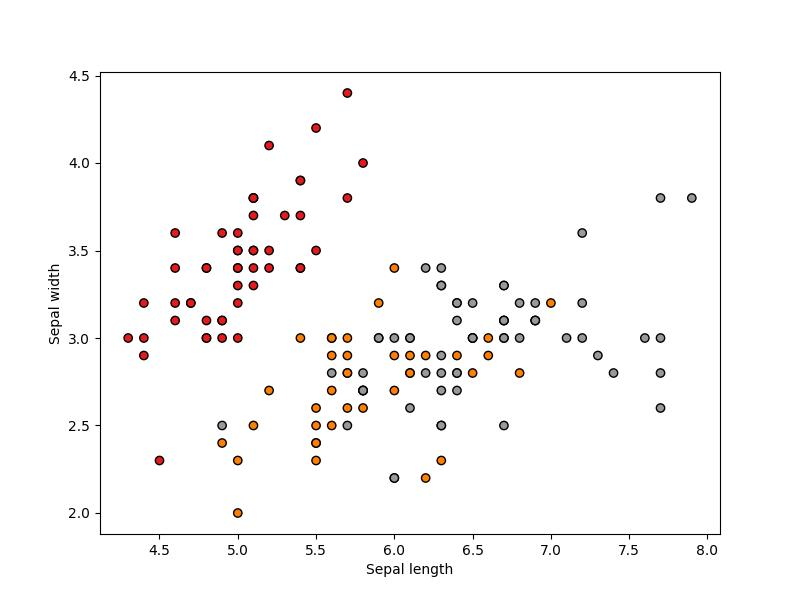
\includegraphics[width=0.8\linewidth]{figures/Ex1_Fig1.jpg}
              \caption{可视化特征 1 和特征 2}
          \end{figure}

          \begin{figure}[H]
              \centering
              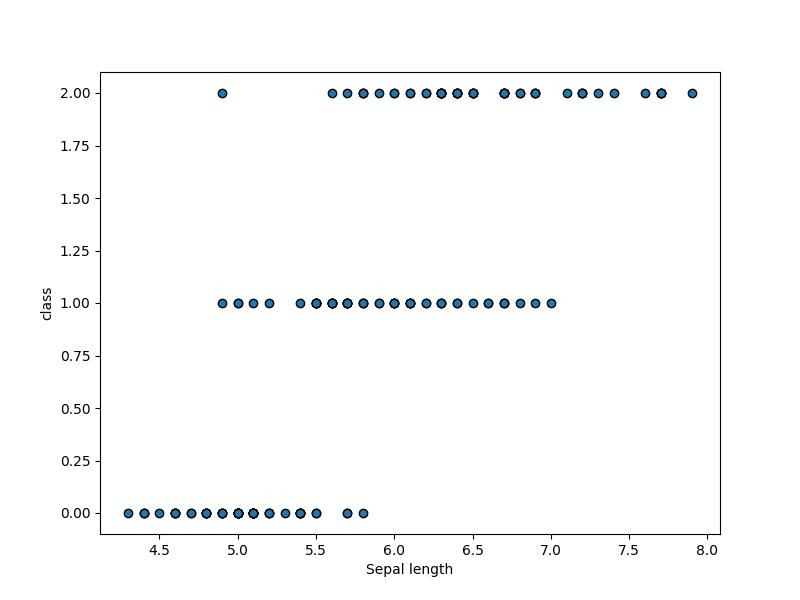
\includegraphics[width=0.8\linewidth]{figures/Ex1_Fig2.jpg}
              \caption{可视化特征 1 和类别 y}
          \end{figure}

          \begin{figure}[H]
              \centering
              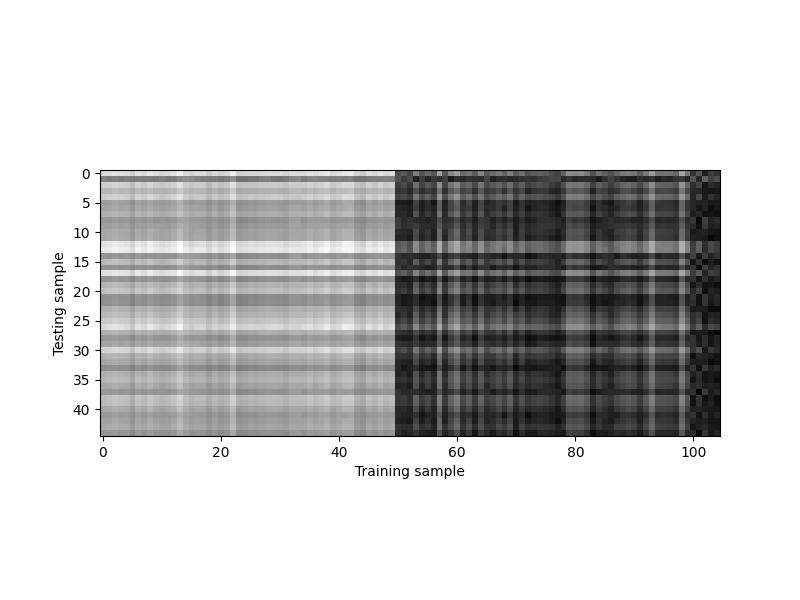
\includegraphics[width=0.8\linewidth]{figures/Ex1_Fig3.jpg}
              \caption{可视化测试集与训练集实例的距离矩阵（灰度越深表示距离越近）}
          \end{figure}

    \item \textbf{kNN分类准确率}

          以7:3划分训练集与测试集，采用欧式距离实现kNN分类。当$k=1$时，模型在测试集上准确率约为73.33\%，表明局部近邻可有效判别鸢尾花类别；但过小$k$易受噪声与异常点影响，存在过拟合风险。

    \item \textbf{5折交叉验证结果}

          通过5折交叉验证对多组$k$值评估，各折准确率稳定、标准差较小，说明数据集分布均匀、模型泛化能力可靠。交叉验证得到各$k$对应平均准确率，可有效规避单次划分带来的评估偏差，为最优$k$选取提供客观依据。
          \begin{table}[H]
              \centering
              \caption{5折交叉验证不同k值的准确率结果}
              \label{tab:knn_cv}
              \small
              \begin{tabular}{cccc}
                  \toprule
                  k值  & 各折准确率                                  & 平均准确率  & 标准差    \\
                  \midrule
                  1   & 1.0000, 1.0000, 1.0000, 0.9524, 0.7619 & 0.9429 & 0.0923 \\
                  3   & 1.0000, 1.0000, 1.0000, 0.9524, 0.7619 & 0.9429 & 0.0923 \\
                  5   & 1.0000, 1.0000, 1.0000, 1.0000, 0.7619 & 0.9524 & 0.0952 \\
                  8   & 1.0000, 1.0000, 1.0000, 1.0000, 0.7619 & 0.9524 & 0.0952 \\
                  10  & 1.0000, 1.0000, 1.0000, 1.0000, 0.7619 & 0.9524 & 0.0952 \\
                  12  & 1.0000, 1.0000, 1.0000, 1.0000, 0.7619 & 0.9524 & 0.0952 \\
                  15  & 1.0000, 1.0000, 1.0000, 1.0000, 0.7619 & 0.9524 & 0.0952 \\
                  20  & 1.0000, 1.0000, 1.0000, 1.0000, 0.7619 & 0.9524 & 0.0952 \\
                  50  & 1.0000, 1.0000, 1.0000, 1.0000, 0.7143 & 0.9429 & 0.1143 \\
                  100 & 0.0000, 0.0000, 0.3810, 0.0000, 0.0000 & 0.0762 & 0.1524 \\
                  \bottomrule
              \end{tabular}
          \end{table}

    \item \textbf{k值大小的影响}

          $k$值直接控制模型复杂度：$k$过小易过拟合，对局部噪声敏感；$k$过大会过度平滑，丢失局部特征导致欠拟合。实验中准确率随$k$增大先升后降，当$k=5$时偏差与方差平衡，分类效果最佳。
          \begin{figure}[H]
              \centering
              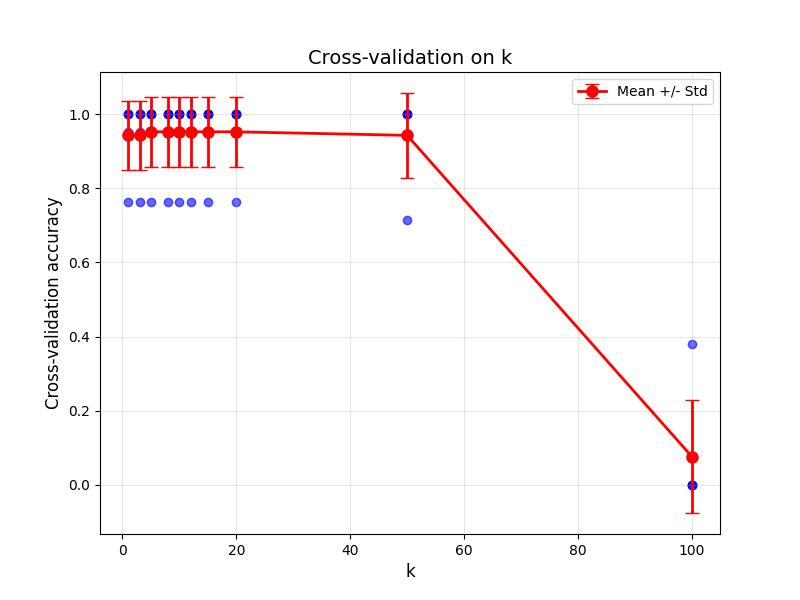
\includegraphics[width=0.8\linewidth]{figures/Ex1_Fig4.jpg}
              \caption{k值大小的影响}
          \end{figure}
\end{enumerate}

\subsection{决策树}
\begin{enumerate}
    \item \textbf{基于信息增益的特征选择}

          实验以信息增益作为特征划分准则，对学生成绩数据集进行最优特征筛选。结果显示，最大信息增益为0.3060，最优划分特征为\textbf{Mid-term test}（期中考试成绩）。

          依据该特征对数据集进行划分，可将样本分为两类：
          \begin{itemize}
              \item 划分值为\textbf{Low}：包含2名学生，期中成绩较低，其中1人未通过考试，1人通过考试，分类不确定性较高；
              \item 划分值为\textbf{High}：包含5名学生，期中成绩较高，全部通过考试，子集纯度较高。
          \end{itemize}
          由此可见，期中考试成绩能够有效区分学生是否通过最终考试，具备较强的分类区分能力。

    \item \textbf{基于信息增益的特征选择}

          为缓解信息增益对取值较多特征的偏好，实验进一步采用信息增益比作为划分准则。结果显示，最大信息增益比为0.3545，最优划分特征仍为\textbf{Mid-term test}。

          划分结果与信息增益准则完全一致，说明该特征不仅具有较高的信息增益，同时特征取值数量均衡，不会因取值分布产生偏好偏差，稳定性与可靠性更强。
          \begin{table}[H]
              \centering
              \caption{决策树特征选择实验结果对比}
              \label{tab:dt_compare}
              \small
              \begin{tabular}{lcc}
                  \toprule
                  指标        & ID3（信息增益）     & C4.5（信息增益比）   \\
                  \midrule
                  最大得分      & 0.3060        & 0.3545        \\
                  最佳划分特征    & Mid-term test & Mid-term test \\
                  Low 子集标签  & Y、N           & Y、N           \\
                  High 子集标签 & 全部 Y          & 全部 Y          \\
                  \bottomrule
              \end{tabular}
          \end{table}
\end{enumerate}

\section{实验总结}
本次实验实现了 k 近邻算法和决策树算法，并在鸢尾花数据集和学生成绩数据集上进行了验证。通过编写代码、调试程序和观察实验结果，我对以下内容有了更深刻的理解：

\subsection{k 近邻算法}
\begin{enumerate}
    \item \textbf{距离度量的选择}：实验对比了欧氏距离和曼哈顿距离，在鸢尾花数据集上两者表现相近，说明对于特征尺度一致且分布良好的数据，距离度量方式的影响较小。
    \item \textbf{k 值的影响}：通过 5 折交叉验证发现，当 \(k=1\) 时模型准确率最高，但随着 \(k\) 增大，准确率逐渐下降且标准差增大。这表明 \(k\) 值过小会导致过拟合（对噪声敏感），\(k\) 值过大会导致欠拟合（过度平滑），选择合适的 \(k\) 值对模型性能至关重要。
    \item \textbf{交叉验证的重要性}：5 折交叉验证有效避免了单次训练集划分带来的评估偏差，为最优 \(k\) 值的选择提供了客观依据，增强了模型的泛化能力评估。
    \item \textbf{数据可视化}：通过 matplotlib 调整散点图的颜色映射、边缘颜色、标记形状等参数，可以更直观地观察数据的分布特征和类别可分性。
\end{enumerate}

\subsection{决策树}
\begin{enumerate}
    \item \textbf{信息熵与条件熵}：信息熵度量数据集的不确定性，条件熵反映已知特征后的剩余不确定性，两者之差即为信息增益。理解这些概念是掌握决策树算法的关键。
    \item \textbf{ID3 与 C4.5 的差异}：ID3 算法使用信息增益作为特征选择准则，容易偏向取值较多的特征；C4.5 算法采用信息增益比进行修正，使特征选择更加公平合理。实验中两者均选择了 Mid-term test 作为最佳特征，说明该特征确实具有较强的分类能力。
    \item \textbf{决策树的划分过程}：通过计算各特征的信息增益（比），选择最优特征进行数据集划分，使得子集纯度不断提高，最终构建出能够正确分类的决策树。
\end{enumerate}

\cite{key2024}

\printbibliography  % 文末输出参考文献列表

% 实验记录

\includepdf[pages=-]{./Record.pdf}

\end{document}